\documentclass[12pt]{scrartcl}
\usepackage[margin=1.2in]{geometry}
\usepackage[french]{babel} % choix de la langue : anglais par défaut
\usepackage[utf8]{inputenc} % choix de l'encodage des caractères : utile pour les accents
\usepackage[T1]{fontenc} 
\usepackage{fancyhdr}
\usepackage{listings}

\lstset{
  xleftmargin=3em,
  literate={->}{$\rightarrow$}{2}
}
%%%%%%%%%%%%%%%%%%%%%%%%%%%%%%%%%%%%%%%%%%%%%%%%%%%%
% Math : les packages classiques : 
\usepackage{amsmath} 
\usepackage{amssymb} 

%%%%%%%%%%%%%%%%%%%%%%%%%%%%%%%%%%%%%%%%%%%%%%%%%%%%
% Algo : 
\usepackage[french]{algorithm2e} 

%%%%%%%%%%%%%%%%%%%%%%%%%%%%%%%%%%%%%%%%%%%%%%%%%%%%
% graphique
\usepackage{graphicx} 
\graphicspath{ {./img/} }

\begin{document}
%%%%%%%%%%%%%%%%%%%%%%%%%%%%%%%%%%%%%%%%%%%%%%%%%%%%%%%%%%%
% DOCUMENT
\pagestyle{fancy}
\rhead{  }
\lfoot{
\includegraphics[scale=0.2]{logounistra}}

\title{%
Simulation d'exécution de programmes parallèles\\
\large } 

\subtitle{ TER. Rapport intermédiaire}
\author{Olga Pigareva\\
M1 SIL} % optionnel

% \date est optionnel : par défaut, date du jour de compilation
% \date{aujourd'hui} % date fixe
% \date{} % pas de date





\maketitle

\newpage

\tableofcontents % facultatif

\newpage % permet de changer de page

\section{La présentation de la problématique dans son contexte}

\subsection{Introduction}
Le sujet de mon travail d'étude et de recherche aborde un domaine d'actualité dans le monde numérique, la programmation parallèle.
La parallélisation de tâches et de processus permet d'augmenter la performance et faire l'exécution d'un programme beaucoup plus rapide. 
C'est pourquoi la programmation parallèle reste un sujet très actuel, même si elle était inventée il y a déjà plusieurs années.\\

La programmation parallèle comprend la résolution d'un problème simultanément par plusieurs processus.
Cela implique l'utilisation d'une seule ressource par plusieurs processus, ce qui nécessite une synchronisation.
De son côté, la synchronisation peut amener à un interblocage qui peut avoir les conséquences indésirables (catastrophiques) pour un programme. \\
Mon travail fait partie d'une recherche visant à caractériser ces interblocages.\\
Dans les parties suivantes, j'expliquerai ce que signifient ces termes.   
%Cela implique Mais quand il y a plusieurs processus qui utilisent la même ressource, l'interblocage peut apparaître. Par exemple, si on a un processus attent un autre processus, qui de sa part attends le première processus. Le programme restera bloqué qui implique plusieurs problèmes. 
%C'est pourquoi on cherche d'éviter et de reconnaître un interblocage le plus tôt possible.

\subsection{Programmes parallèles}

Les programmes parallèles permettent de créer les activités qui peuvent exécuter les instructions indépendamment. 
Souvent ces activités ont besoin d'acceder aux mêmes ressources. 
Pour ne pas avoir les résultats imprévus lors de modification de données par les processus différents, les ressources sont synchronisées. 
Cela veut dire que les processus peuvent acceder aux données chacun à son tour. 
Pour attendre la libération de données ou la fin d'instructions d'un processus, un programme parallèle utilise les horloges qui sont les barrières de synchronisation.
\newpage

\subsection{Interblocage}

Le problème d'interblocage apparaît quand chaque processus attend un autre pour se terminer et finalement aucun peut acceder à la ressource.
Par conséquent, le programme reste bloqué.\\

Par exemple, sur la Figure 1, le processus P1 attend la fin de processus P2 pour acceder à R1. Et P2, de son côté, attend la fin de P1 pour acceder à R2. Tous les deux processus restent bloqués.\\

\begin{figure}[h]
  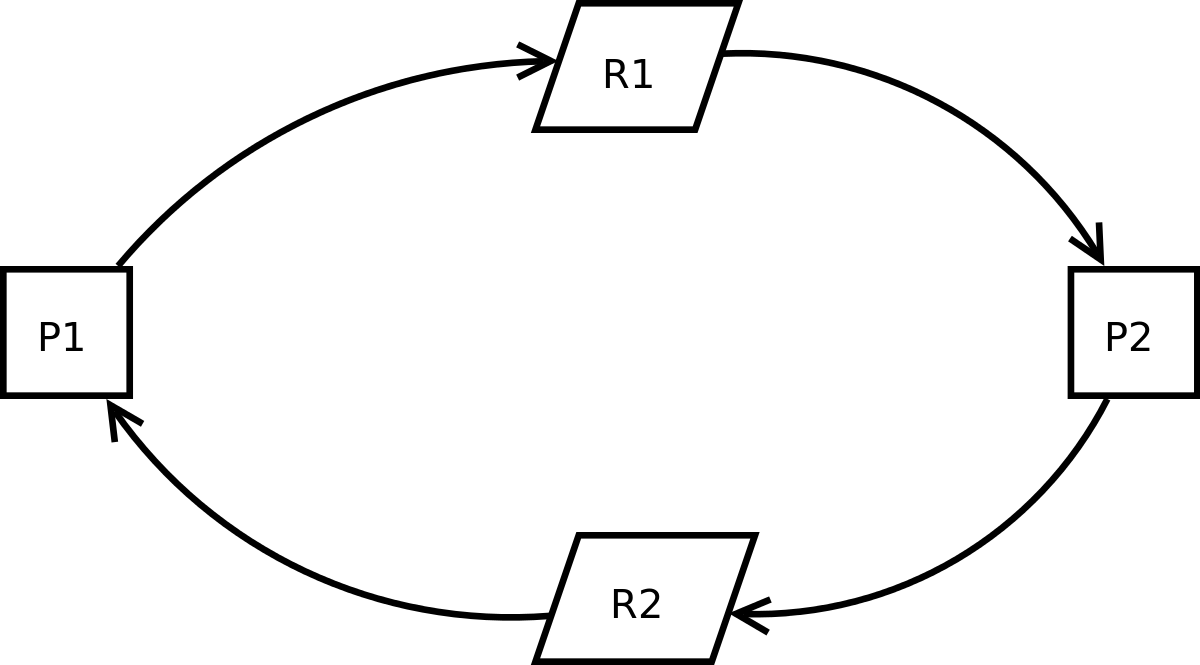
\includegraphics[scale=0.2]{deadlock}
  \centering
  \caption{Exemple d'interblocage}
  \centering
\end{figure}

Souvent pour les programmes avec plusieurs processus et plusieurs ressources, il est difficile de contrôler l'absence d'interblocages, surtout avec la liberté et puissance offertes par la synchronisation.
D'où l'intérêt de reconnaître ces interblocages automatiquement le plus tôt possible, à savoir, éventuellement, lors de la compilation du programme.

\newpage

\subsection{Problème et objectifs}

Est-il possible de définir un interblocage pendant l'étape de compilation?\\

 Pour répondre à cette question, l'idée est de commencer par créer une version simplifiée d'un langage parallèle en prenant un langage X10 comme un exemple.
 Le compilateur doit reconnaître juste les instructions qu'on a besoin pour créer plusieurs activités parallèles (boucles, conditions, création de nouveaux processus et horloges).\\
 L'exemple de tel programme est représenté par la Figure 2.

 \begin{figure}[h]
  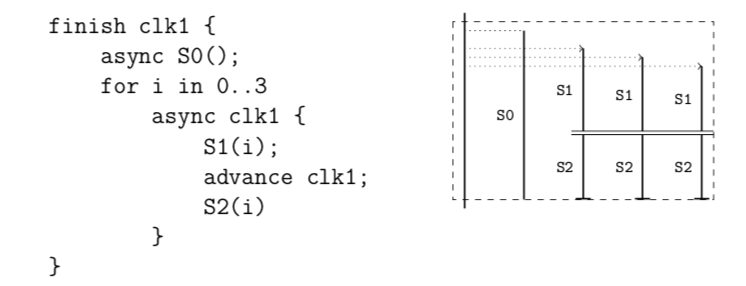
\includegraphics[scale=1]{program}
  \centering
  \caption{Exemple d'un programme parallèle}
  \centering
\end{figure}

 Après avoir implémenté un langage qui permet de créer plusieurs activités parallèles avec la synchronisation, il doit être possible de visualiser l'état de toutes les activités au moment d'interblocages.
 Pour cela, il faut créer une machine virtuelle qui va être capable de simuler l'exécution de programmes parallèles et donner une liste d'activités. \\

 \newpage
 
\section{La liste des tâches déjà effectuées}

\subsection{Le travail réalisé}
\begin{itemize}
 \item Installation de librairies et IDE pour le langage de programmation \textbf{X10} sur mon ordinateur.\\ Premièrement, il fallait préparer l'environnement de travail.
 \item Lecture de la documentation et d'autres ressources sur l'interblocage et programmes parallèles.
 \item Exécution de différents programmes test X10 pour comprendre le problème et voir comment il fonctionne. 
 \item Implementation d'un compilateur inspiré par le langage X10 à l'aide de Lexer et parser (Lex et Yacc).
 \item Génération d'un arbre de la syntaxe abstraite (AST en anglais).
\end{itemize}



\section{Le planning prévisionnel des tâches à réaliser}
\begin{description}
  \item[mars] Implémentation de la simulation d'exécution du programme et captures de traces d'exécution.
  \item[avril] Implémentation de visualisation des traces d'execution ou de systèmes mathématiques permettant de détecter un interblocage.
  \item[mai] Rédiger un rapport avec le bilan de résultats atteints.
\end{description}


\newpage

\section{Choix d'implémentation et différentes étapes}

\subsection{Grammaire}
\begin{lstlisting}
  program -> list_stmt

  stmt -> instruction ';' 
          |   FOR ID '=' range block 
          |   IF '(' affine ')' block  
          |   IF '(' affine ')' block ELSE block
          |   FINISH '(' clocks ')' block
          |   FINISH block
          |   ASYNC '(' clocks ')' block
          |   ASYNC block
          |   ADVANCE ID ';'

  list_stmt -> list_stmt stmt | stmt

  instruction -> ID

  clocks -> /*empty*/
          |   clocks ',' ID
          |   ID

  block -> \{' list_stmt '\}'
          |   stmt

  range -> affine RANGE affine

  affine -> affine '+' affine
    |   affine '-' affine
    |   affine '/' affine
    |   affine '*' affine
    |   affine COMP affine
    | '(' affine ')'
    | ID
    | NUMBER
\end{lstlisting}

\newpage

\subsection{Génération du code intermédiaire}
\begin{description}
  \item[EVAL]

  \item[FINISH]
  - créer une nouvelle structure finish
  - la rajouter dans une pile de finish de l'activité en cours

  \item[CLOCK_CREATE]
  - créer une nouvelle structure clock
  - ajouter l'activité en cours dans la pile 'registered' régistré avec ce clock
  - rajouter ce clock dans une pile de clocks de l'activité en cours
  - rajouter ce clock dans une pile de clocks de finish de l'activité en cours

  \item[END_FINISH]:
  - 
  \item[ASYNC_SUITE]: 
  //goto
  - modifier le compteur du programme sur la ligne marquée dans le code
  \item[CLOCK_REGISTER]:
  - rajouter le clock dans une pile de clocks de l'activité en cours
  - ajouter l'activité en cours dans la pile 'registered'  régistré avec ce clock
  \item [END_ASYNC]   
  \item [ADVANCE]
\end{description}

\newpage      
\begin{thebibliography}{9}
  \bibitem{sujet} 
  Alain Ketterlin.
  \textit{La présentation de sujet de TER}. 
   
  \bibitem{parallel} 
  Agarwal Shivali, Barik Rajkishore, Sarkar Vivek, Shyamasundar R.K.\\
  \textit{May-happen-in-parallel analysis of X10 programs}.
  Proceedings of the ACM SIGPLAN Symposium on Principles and Practice of Parallel Programming (2007), PPOPP.
   
  \bibitem{x10} 
  Vijay Saraswat, Bard Bloom, Igor Peshansky, Olivier Tardieu, and David Grove
  \textit{X10 Language Specification}. 
  Version 2.6.2

  \bibitem{deadlock} 
  Composing Programs: Parallel Computing,
  \\\texttt{https://composingprograms.com/pages/48-parallel-computing.html}
  \end{thebibliography}
 \addcontentsline{toc}{section}{Références}
 \bibliographystyle{alpha}

\end{document} 

